\section{Algorithms}\label{sec:algorithms}
In this section, we introduce algorithms for statistical analysis of networks. Section \ref{sec:single_algo} provides an overview of algorithms for a single graph and Section \ref{sec:multi_algo} provides an overview of algorithms designed for multiple graphs. 

% Important TODO: Check consistency of the subindex notation. Here U_d is indicating something different than in the previous section (rows of U vs a matrix with d columns?)
% Another important TODO: The definition of ASE is wrong, A is not equal to USU^T, that is the truncation to its first d eigenvectors. I'm going to change it but please make sure that there are not problems with this in the rest of the paper.


\subsection{Single Graph Algorithms}\label{sec:single_algo}
\subsubsection{Adjacency and Laplacian Spectral Embedding (ASE, LSE)} \label{sec:ase}
Given an undirected graph with adjacency matrix $\A$, the adjacency spectral embedding ($\ase$) and Laplacian spectral embedding ($\lse$) construct a representation of the vertices of the graphs into $d$ dimensions via its eigendecomposition, given by
$\A = \mathbf{U}\mathbf{S}\mathbf{U}^\top$
where $\mathbf{U}\in\RR^{n\times n}$ is the orthogonal matrix of eigenvectors and $\mathbf{S}\in\RR^{n\times n}$ is a diagonal matrix containing the eigenvalues of $\A$ ordered by magnitude, such that $|\mathbf{S}_{11}|\geq |\mathbf{S}_{22}| \geq \ldots \geq |\mathbf{S}_{nn}|$. 
 The $\ase$ of the graph into $\RR^{d}$ is defined as $\ase(\A)=\hat{\X}= \hat{\mathbf{U}}|\hat{\mathbf{S}}|^{1/2}$, where $\hat{\mathbf{U}}\in\RR^{n\times d}$ contains the first $d$ columns of $\mathbf{U}$, which correspond to the largest eigenvectors, and $\hat{\mathbf{S}}\in\RR^{d\times d}$ is the submatrix of $\mathbf{S}$ corresponding to the $d$ largest eigenvalues in magnitude. The $\lse$, of $\A$ is defined in a similar manner using the normalized Laplacian of the graph defined as $\mathbf{L} = \mathbf{D}^{-1/2}\A\mathbf{D}^{-1/2}$ where $\mathbf{D} \in\RR^{n\times n}$ is a diagonal matrix with entries $\mathbf{D}_{ii}=\sum_j\A_{ij}$. Then, the $\lse$ of the graph is given by $\lse(\A)=\ase(\mathbf{L})=\tilde \X\in\RR^{n\times d}$.
% TODONE: I changed \hat{X} to \tilde{X} for LSE to distinguish them from each other (that's what other papers commonly write them). Please check if it needs to be changed somewhere else.
% TODO@ja - corrected. Underscore means rows

% TODONE: Here the definition is also wrong, I fixed it but please check the rest
In the case of directed graphs, the eigendecomposition is not available since adjacency matrix is not symmetric, so instead we use the singular value decomposition of the adjacency matrix as $\A=\mathbf{U}\mathbf{S}\mathbf{V}^\top$, where $\mathbf{U},\mathbf{V}\in\RR^{n\times n}$ are orthogonal matrices containing the left and right singular vectors, and $\mathbf{S}\in\RR^{n\times n}$ is a non-negative diagonal matrix with the singular values. 
The $\ase$ of a directed graph results in two different latent position matrices $\hat{\X}= \hat{\mathbf{U}}\hat{\mathbf{S}}^{1/2}$ and $\hat{\Y}= \hat{\mathbf{V}}\hat{\mathbf{S}}^{1/2}$, denoted \textit{in} and \textit{out} latent positions, respectively, where $\hat{\mathbf{U}},\hat{\mathbf{V}}\in\RR^{n\times d}$ contain the $d$ columns of $\mathbf{U}$ and $\mathbf{V}$ corresponding to the $d$ leading singular vectors, and $\hat{\mathbf{S}}$ is the submatrix of $\mathbf{S}$ containing the $d$ leading singular values. 
While there exists many definitions for directed normalized Laplacian, we define it as $\mathbf{L} = \mathbf{D}^{-1/2}\A\mathbf{O}^{-1/2}$ where $\mathbf{D}_{ii} =\sum_j\A_{ij}$ and  $\mathbf{O}_{ii} =\sum_j\A_{ji}$ are the in and out degree diagonal matrices \cite{rohe2016co}. The $\lse$ of directed graph processed similarly to that of directed $\ase$. 

Spectral embedding is the first step in many subsequent inference tasks. For example, spectral clustering for community detection (Section \ref{sec:clustering_single}) can be achieved via Gaussian Mixture modeling on $\hat \X$ from either $\ase$ or $\lse$. The resulting cluster assignments can further be used to estimate the parameters for \textit{a posteriori} $\sbm$. 

For real data, the true embedding dimension $d$ is often not known and must be estimated. A general methodology for choosing the embedding dimension $d$ is to examine the scree plot of the singular values of $\A$ and look for an ``elbow'' or a ``big gap''. While many methods for choosing the threshold exist \cite{jackson2005user,chatterjee2015matrix}, we consider the method in \cite{zhu2006automatic} when applying any spectral embeddings in real data. Given $\A= \mathbf{U}\mathbf{S}\mathbf{U}^\top$ for either $\ase$ or $\lse$, the eigenvalues in $|\mathbf{S}|$ are used to estimate the embedding dimension $\hat d$ by maximizing the profile likelihood function, which determines the magnitude of the ``gap'' after first $d$ largest eigenvalues. Multiple elbows can be found by discarding the $\hat d$ number of largest eigenvalues and repeating the process with the remaining eigenvalues. For applications in connectomics, we only consider $\ceil{\log{n}}$ largest eigenvalues as input to the profile likelihood function and take the second elbow as the estimate of $\hat d$.
% \begin{align*}
%     \hat d &= \argmax_d \mathrm{ProfileLikelihood}_S(d)
% \end{align*}
% TODONE: I don't think it adds any value to display an equation like this if the exact form of the profile likelihood function is not going to appear. Maybe delete and just mention that d hat maximizes the profile likelihood (i.e. the same thing but with words).

% TODONE mention ZG(2) explicitly please, as well as log(n) as the upperbound on d, or whatever other tricks we do. this will be the only place that stuff is ever actually written down.

\subsubsection{Diagonal Augmentation}\label{sec:diag-aug}
Many connectomes have no self-loops, resulting in all zero in the diagonal entries of the adjacency matrices. When computing spectral embeddings of graphs, the zero diagonal results in increased errors in estimation \cite{tang2018connectome}. Furthermore, the sum of eigenvalues of the adjacency matrices is zero, leading to an indefinite matrix, which violate assumptions of the statistical models such as $\rdpg$. 

Diagonal augmentation ($\sct{diag-aug}$) is a method for imputing the diagonals of adjacency matrices from graphs with no self-loops \cite{marchette2011vertex,tang2018connectome,scheinerman2010modeling}. The diagonals are imputed with with the average of the non-diagonal entries of each row, which corresponds to the degree of each vertex divided by $n-1$. In the case of directed graphs, the average of in and out degree is used. Specifically, the diagonal augmented adjacency matrix is defined as $\tilde \A = \A + \tilde\D$ where $\A\in\RR^{n\times n}$, $\tilde \D \in\RR^{n\times n}$ is a diagonal matrix with entries $(\mathbf{A}\vec 1^\top + \vec 1\mathbf{A}) /2(n-1)$ where $\vec 1 \in\RR^n$ is a row vector of ones. To achieve best embedding estimation, the diagonal entries of adjacency matrices should be imputed prior to $\ase$ (in $\lse$, the diagonals are imputed via the normalized Laplacian).

\subsubsection{Pass-To-Ranks (PTR)}
Connectomes have often weighted edges, which can take on arbitrary values. Rescaling and normalizing the edge weights has been shown to increase reliability and can improve estimation of spectral embeddings \cite{Kiar188706}. Pass-to-ranks ($\ptr$) is a method for rescaling the \textit{positive} edge weights such that all edge weights are between 0 and 1, inclusive. 

Given an adjacency matrix $\A \in \Real^{n\times n}$, let $R(\A_{ij})$ be the ``rank'' of $\A_{ij}$, that is, $R(\A_{ij}) = k$ if $\A_{ij}$ is the $k^{th}$ smallest number in $\A$. The rescaled adjacency matrix, $\Tilde{\A}$, is defined as follows:
\begin{align*}
    \Tilde{\A}_{ij} &= \begin{cases}
    \frac{R(\A_{ij})}{|E|} & \text{if $\A_{ij} > 0$},\\
    0 & \text{otherwise},
    \end{cases}
\end{align*}
where $|E|$ is the number of non-zero edges. Ties in rank are broken by averaging the ranks. For spectral embedding of weighted connectomes, they are first normalized via $\ptr$, then the diagonals are imputed via $\sct{diag-aug}$ prior to $\ase$ ($\sct{diag-aug}$ is skipped for $\lse$). 

\subsubsection{Spectral Clustering for Community Detection} \label{sec:clustering_single}
One of the most common uses of spectral clustering is for community detection, in which the vertices with similar connectivity patterns are grouped together. Given the embeddings of a graph from either $\ase$ or $\lse$, classical Euclidean clustering of $\hat{\X}$ results in community structure. Central limit theorems for spectral embeddings of many statistical models (e.g. $\sbm$, $\rdpg$) suggest Gaussian Mixture modeling ($\gmm$) for clustering (see Appendix \ref{sec:theory_single}).

The true number of clusters, $K$, is often not known in real data, but can be estimated by maximizing likelihood functions penalized by model complexity. Commonly used functions include Bayesian Information Criterion ($\bic$), Akaike Information Criterion ($\sct{AIC}$), and Minimum Description Length ($\sct{MDL}$) \cite{akaike1974new, schwarz1978estimating, rissanen1978modeling}. By default, we use penalized likelihood via $\bic$ to estimate $K$ \cite{priebe2019two}. In practice, various covariance types and initialization methods for $\gmm$, and number of clusters are swept over to compute best estimated number of cluster, $\hat K$ \cite{athey2019autogmm, scrucca2016mclust}.



\subsection{Multiple Graph Algorithms}\label{sec:multi_algo}
\subsubsection{Omnibus Embedding}\label{sec:omni}
Consider a sample of $m$ observed graphs $\mathcal{G}^{(1)}, \mathcal{G}^{(2)}, \ldots, \mathcal{G}^{(m)}$  and their associated adjacency matrices, $\A^{(1)}, \A^{(2)}, \ldots, \A^{(m)}\in\RR^{n\times n}$ with $n$ vertices that are identical and shared across all graphs. Under the $\jrdpg$ model, $\omni$ is a consistent method (see Appendix \ref{sec:theory_multi}) for simultaneously estimating the latent position matrices for each graph by computing the spectral embedding into $d$-dimensions on the omnibus matrix, $\mathbf{O}\in\RR^{nm\times nm}$, as defined below
\begin{align*}
\mathbf{O} &= 
\begin{bmatrix}
\A^{(1)} & \frac{1}{2}\parens*{\A^{(1)}+\A^{(2)}} & \cdots & \frac{1}{2}\parens*{\A^{(1)}+\A^{(m)}}\\
\frac{1}{2}\parens*{\A^{(2)}+\A^{(2)}} & \A^{(2)} & \cdots & \parens*{\A^{(2)}+\A^{(m)}}\\
\vdots & \vdots & \ddots & \vdots\\
\frac{1}{2}\parens*{\A^{(m)}+\A^{(1)}} & \frac{1}{2}\parens*{\A^{(m)}+\A^{(2)}} & \cdots & \A^{(m)}
\end{bmatrix}
\end{align*}
The embeddings gives the matrix
\begin{align*}
    \hat{\mathbf{Z}} &= \ase(\mathbf{O}) = 
    \begin{bmatrix}
    \hat{\X}^{(1)}\\
    \hat{\X}^{(2)}\\
    \vdots\\
    \hat{\X}^{(m)}
    \end{bmatrix}\in\RR^{mn\times d}
\end{align*}
where the first $n$ rows are the latent positions corresponding to $\A^{(1)}$, so on and so forth. 

\subsubsection{Multiple Adjacency Spectral Embedding (MASE)}\label{sec:mase}
$\mase$ is a consistent method for estimation (see Appendix \ref{sec:theory_multi}) of underlying parameters for each graph under the $\cosie$ model \cite{arroyo2019inference}. $\mase$ is a is a three step process:
\begin{enumerate}
    \item Each adjacency matrix, $\A^{(i)}$, is embedded into $d$ dimensions via $\ase$, and the matrix $\hat{\mathbf{U}} = \bracks*{\ase(\A^{(1)}), \ase(\A^{(2)}), \ldots, \ase(\A^{(m)})} \in \RR^{n\times dm}$ is the concatenated matrix of spectral embeddings.
    \item Calculate the singular value decomposition of $\hat{\mathbf{U}}=\mathbf{V}\mathbf{S}\mathbf{W}^\top$, and let  $\hat{\V} \in \RR^{n\times d}$ be the matrix containing  the $d$ singular vectors corresponding to $d$ largest singular values. $\hat\V$ is the estimated shared common subspace matrix.
    \item  Individual matrices are estimated via $\hat{\mathbf{R}}^{(i)} = \hat{\V}^\top\A^{(i)} \hat{\V}$ where $\hat{\mathbf{R}}^{(i)}\in \RR^{d \times d}$.
\end{enumerate}

\subsubsection{Spectral Clustering for Community Detection} \label{sec:clustering_multi}
Similar to the procedure described in Section \ref{sec:clustering_single}, one can also perform spectral clustering in the multi-graph setting. Clustering is performed on the the average latent position matrix, $\bar{\X} \coloneqq \frac{1}{m}\sum_{i=1}^m \hat{\X}^{(i)}$, in $\jrdpg$ model and the vertex subspace matrix, $\hat{\V}$ in $\cosie$ model. The clustering procedure proceeds identically as described in Section \ref{sec:clustering_single}. %Figure \ref{fig:exp3_latent_positions} visualizes the embeddings and the results from spectral clustering under $\jrdpg$ and $\cosie$ models.

% \begin{figure}
%     \centering
%     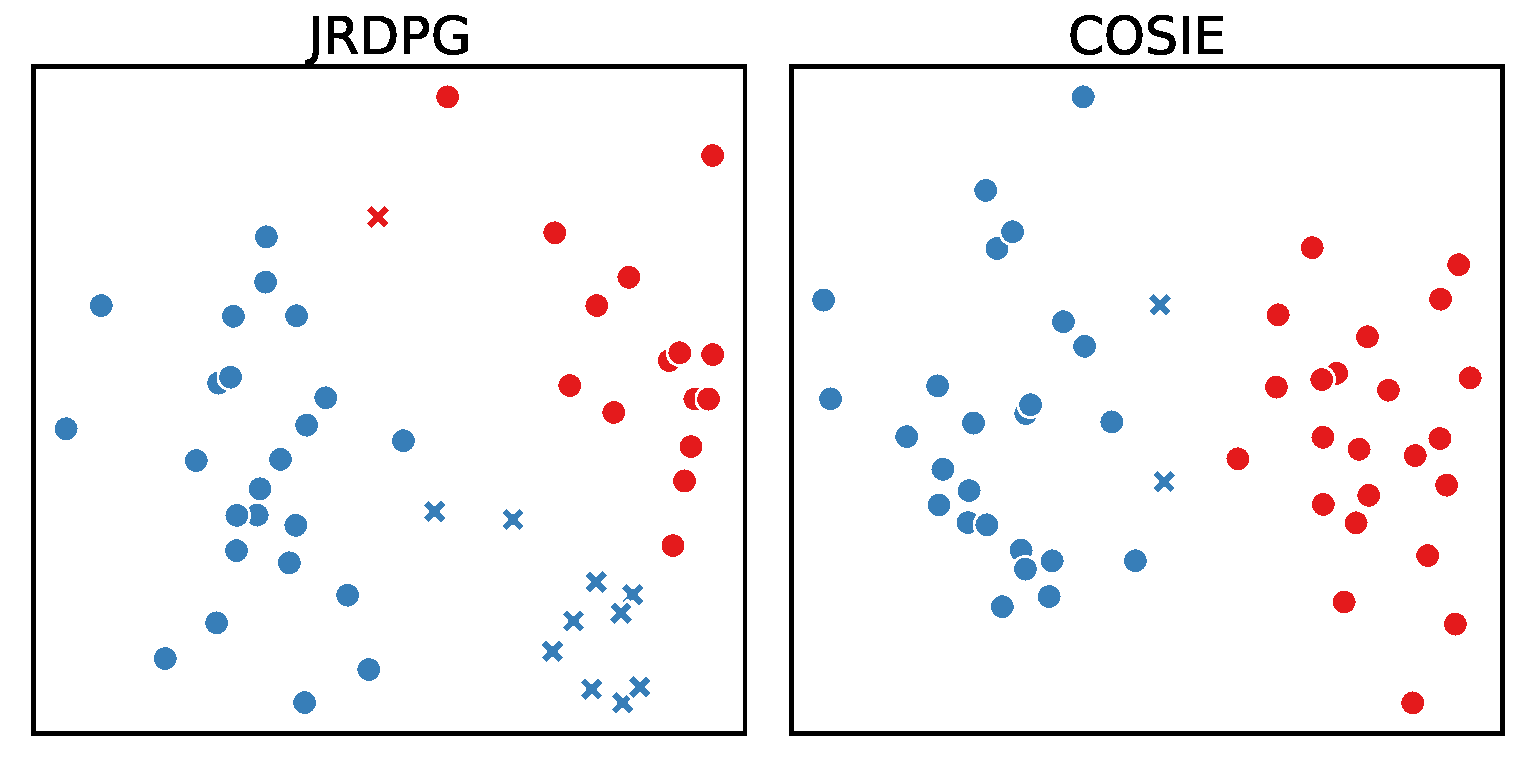
\includegraphics[width=0.65\textwidth]{figures/dnd/exp3_latent_positions.pdf}
%     \caption{\textbf{Visualization of vertices in 2D space in $\jrdpg$ and $\cosie$ models.} Total of $m=100$ $\mathsf{kidney-egg}$ $\sbm$ with $a=0.5$ and $b=0.65$ are sampled. The networks are embedded into $d =2$ dimensions, and the mean estimated latent position matrix, $\bar{\X}$, and the estimated vertex subspace matrix, $\hat{\V}$, are shown. The colors corresponds to the estimated community assignments obtained from 2-cluster $\gmm$. Dots represent correctly labeled vertices and $x$ markers represent incorrectly labeled vertices. As effect size increases, the separation between two communities increase, and misclassification rate decreases.}
%     \label{fig:exp3_latent_positions} % TODO must define 'effect size' here, or not use the term.
%     % TODO: would it be possible to put the embedding for different sizes of graphs to see the effect of increasing n? If it is too much work, I think it is fine, but the plot doesn't look  obviously clustered, so maybe showing that increasing n makes the points to be closer to its mean will be more informative
% \end{figure}

\subsubsection{Seeded Graph Matching (SGM)} \label{sec:sgm}
Consider two graphs $\mathcal{G}^{(1)}$ and  $\mathcal{G}^{(2)}$ with $n$ vertices and their associated adjacency matrices $\A$ and $\B$, respectively. The graph matching problem seeks to find an alignment of nodes between these two graphs that minimizes the number of edge disagreements. Formally, it is defined as the following optimization problem:
% TODONE the below formalization is obtuse.  use the norm formulation like i did in FAQ please, || A - Q B Q\T ||
% TODO we already used P above, so let's use Q for permutation matrix?
\begin{align}
    \min & %{\ \text{-trace}({\A}\Pbf\B^\top \Pbf^\top)} 
    ~\norm*{\A\Pbf - \Pbf\B}_F^2
    \label{eq:GMP}\\
    \mbox{s.t.} & {~\Pbf  \in \mathcal{P}} \nonumber
\end{align}
where $\mathcal{P}$ is the set of permutation matrices in $\RR^{n \times n}$.
% TODONE i think sgm is a modification of GM, not the algorithm FAQ which solves GM.  
Seeded graph matching ($\sgm$) is a modification of the graph matching algorithm, allowing for the specification of seed sets $W_1$, $W_2$ with seeding $\psi : W_1 \rightarrow W_2$, and solved via fast approximate quadratic assignment ($\sct{FAQ}$) \cite{vogelstein2015fast}.
As the seeded graph matching problem is computationally intractable, $\sgm$ provides an approximate solution by relaxing the feasible region from $\mathcal{P}$ to $\mathcal{D}$, the set of doubly stochastic matrices. The algorithm is provided below:
\begin{enumerate}
    \item Initialize at some $\Pbf^{(0)} \in \mathcal{D}$, where $\mathcal{D}$ is the set of doubly stochastic matrices. Typically, initialization is chosen as $\Pbf^{(0)} = \vec{1}\vec{1}^\top / n$, where $\vec{1}$ denotes the $n$-vector of all ones.
    \item \textbf{while} stopping criteria not met \textbf{do}
        \begin{enumerate}
            \item Compute the gradient $\Delta f\left(\Pbf^{(i)}\right)$
            \item Compute the search direction $\Q^{(i)} \in \argmax{\left(\trace{\Q^{T} \Delta f(\Pbf^{\left(i\right)})}\right)}$ via Hungarian Algorithm
            \item  Compute step size $\alpha^{(i)} \in \argmax(f(\alpha^{(i)} \Pbf^{(i)} + (1 - \alpha^{(i)}) \Q^{(i)})) $
            \item Update $\Pbf^{(i+1)} := \alpha^{(i)} \Pbf^{(i)} + (1 - \alpha^{(i)}) \Q^{(i)}$
        \end{enumerate}
    \item Compute $\hat{\Pbf} \in \argmax\left(\trace{\Pbf^{\top} \Pbf^{(final)}}\right)$ via Hungarian Algorithm
\end{enumerate} 
